\pagestyle{circuito}
\label{circuito}

\begin{textblock*}{5.625in}(0pt,0pt)%
\vspace*{-3.5cm}
\hspace*{-2.77cm}\includegraphics*[width=175.2mm]{./propagandas/CIRCUITO.pdf}
\end{textblock*}

\pagebreak %AS ARTES DO COVER


\begin{center}
\hspace*{-3.6cm}\raisebox{5cm}{\rotatebox[origin=t]{90}{\huge\Formular{\textbf{Lançamento}}}}
\hspace*{3.1cm}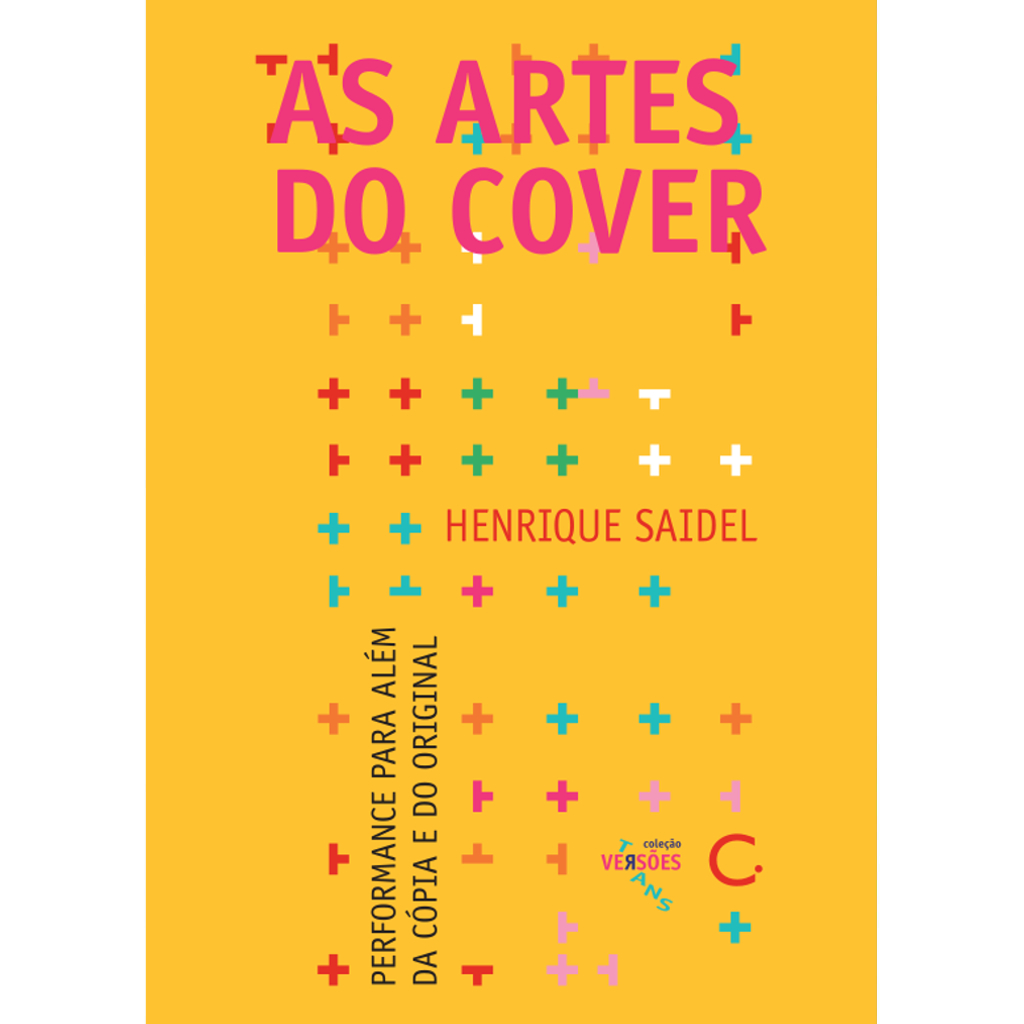
\includegraphics[width=74mm]{./grid/cover.jpg}
\end{center}

\hspace*{-7cm}\hrulefill\hspace*{-7cm}

\medskip

\noindent{}Noção de origem, original, único, essência originária. O que é afirmado ao dizermos que algo é original? Desde Aristóteles já se sabe que a imitação – ou mímesis – deveria recriar a potência de vida e não sua forma. É com base nesse pensamento que o autor pode afirmar que o cover é também uma criação, mesmo relacionado à sua base precedente e sem qualquer hierarquia preestabelecida. O cover inventa outro original.
A origem passa então a ser um início que se recria em {\slsc{continuum}}, sempre presentificada em ato, um simulacro com força de raiz: a presente obra repensa a noção de presente e de presença através do cover. Uma presença pensada como acontecimento subversivo, que borra as linhas que separam o “mesmo” do “diferente”, o “original” do “simulacro”, e concretiza passado e presente no mesmo ato. O cover como pulso da repetição do dessemelhante, como inventividade plena. Quem veio primeiro, o ovo ou a galinha? A leitura de {\slsc{As artes do cover}}, escrito pelo diretor de teatro, performer, professor, curador e crítico Henrique Saidel, nos permite vê"-los juntos em ato, no mesmo tempo"-espaço de criação.

\vfill

\hspace*{-.4cm}\begin{minipage}[c]{.5\linewidth}
\small{
{\Formular{\textbf{
\hspace*{-.1cm}\hlc[lightyellow]{Editora: Circuito}\\
Título: As artes do cover\\
Autor: Henrique Saidel\\ 
ISBN: 978-85-9582-049-4\\
Páginas: 352\\
Formato: 14x21cm\\
Preço: R\$ 55,00\\
Disponibilidade: Disponível
}}}}
\end{minipage}

\pagebreak %TODOS OS LUGARES


\begin{center}
\hspace*{.5cm}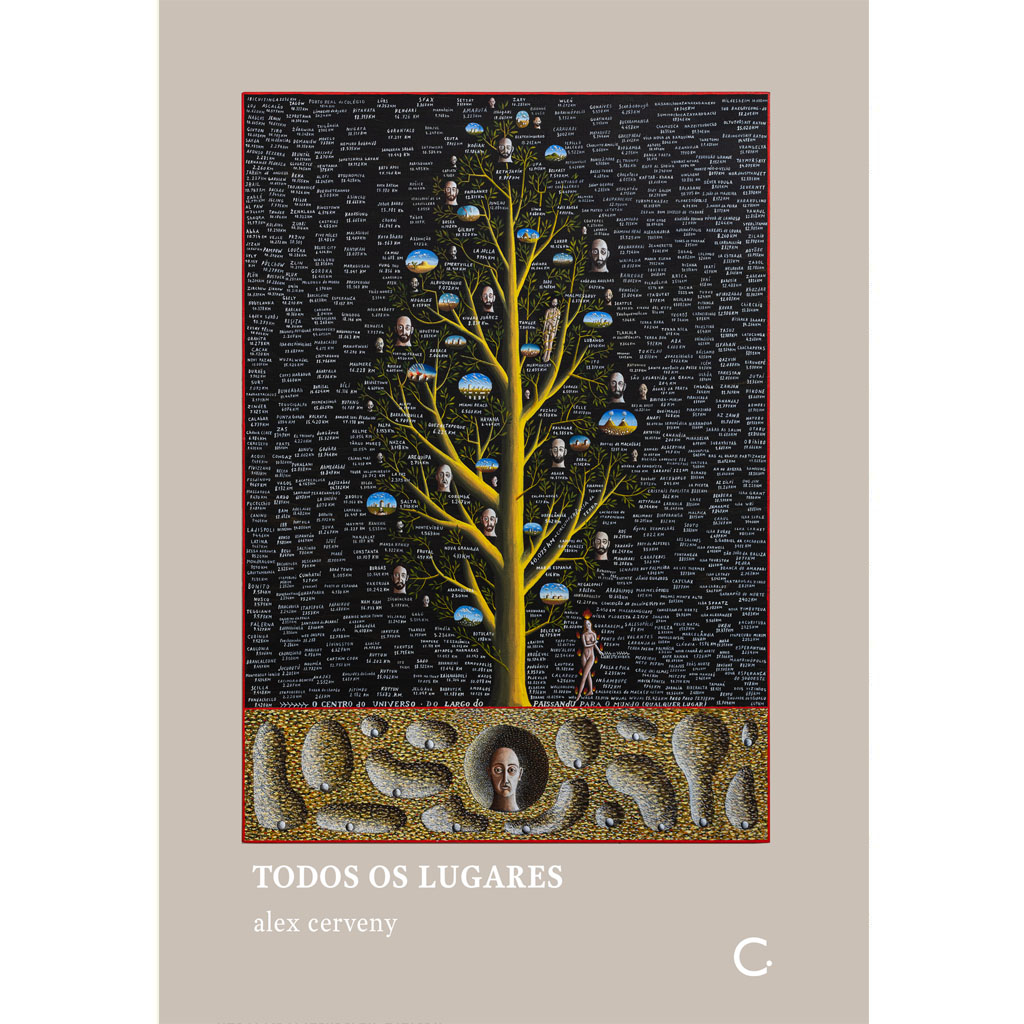
\includegraphics[width=74mm]{./grid/lugares.jpg}
\end{center}

\hspace*{-7cm}\hrulefill\hspace*{-7cm}

\medskip

\noindent{}{\slsc{Todos os lugares}} trata"-se de um glossário, escrito e ilustrado pelas talentosas mãos de Alex Ceverny, artista plástico, desenhista, gravador, escultor, ilustrador e pintor. Percorre cidades e lugares onde esteve, tecendo comentários “de uma observação ferina e fértil, aguda sensibilidade e humor irônico quase mordaz”, engendrando assim “espaços e situações singulares, quase oníricos e belos; mundos solitários com os quais de algum modo sonhamos e de alguma forma aspiramos habitar”, conforme escreve Renato Rezende no prefácio.

Um dos mais notáveis artistas brasileiros da atual geração, Ceverny produz em suas viagens peregrinações e inflexões sobre si próprio, dividindo uma vida rica e cuidadosamente enlaçada entre imagem e escrita, entre “riscos, traços e viagens”. Belo e singular, o livro conta também com prefácio do curador Renato Rezende e posfácio do escritor e filósofo Rodrigo Petronio.

\vfill

\hspace*{-.4cm}\begin{minipage}[c]{.5\linewidth}
\small{
{\Formular{\textbf{
\hspace*{-.1cm}\hlc[lightyellow]{Editora: Circuito}\\
Título: Todos os lugares\\
Autor: Alex Cerveny\\ 
ISBN: 978-85-9582-050-0\\
Páginas: 190\\
Formato: 16x23cm\\
Preço: R\$ 80,00\\
Disponibilidade: Disponível
}}}}
\end{minipage}

\pagebreak

\vspace*{1.5cm}

\noindent{}{\nohyphens{\LARGE{Entre todos os lugares\\\noindent{}{\large\slsc{Riscos, traços, viagens: é pelo desenho que o pensamento encarnado\\ em uma pintura se dá a perceber, que o pensamento se une ao sensível}}}}}

\bigskip

\hfill{}\scalebox{.8}{RENATO REZENDE}

\bigskip
\bigskip
\bigskip


Sobretudo um poeta, o pintor e gravurista Alex Cerveny é dotado de imaginação ferina e fértil, aguda sensibilidade e humor irônico e quase mordaz. Espaços e situações singulares, quase"-oníricos e belos, mundos solitários com os quais de algum modo sonhamos e de alguma forma aspiramos habitar: há algo na estranheza das imagens do artista com que nos identificamos atavicamente, e suas superfícies planas — raramente faz uso de perspectiva, mas adota efeitos de sombra e luz, criando volumes ilusórios — funcionam como uma espécie de espelho de algum nosso mundo interior silencioso (mas sempre à beira de dizer algo) e perdido, possivelmente na infância.

Fundamentalmente lírico e fabular em seu afã elaborador, como um criador de mitos — não seria este fundamentalmente o lugar do artista? —, compreendendo perfeitamente e comentando com astúcia e certa compaixão a complexidade e sublimidade do mundo contemporâneo, é capaz de transubstanciá"-lo em narrativas plenas de espiritualidade, sentido e humanidade.

O êxito de sua complexa linguagem poética é também fruto da salutar distância que Alex Cerveny sempre soube manter, escolhendo o caminho de uma trajetória praticamente autodidata, dos imperativos do mercado, e de sua autonomia em relação aos movimentos geracionais. Muito embora possamos situá"-lo historicamente como integrante da fecunda geração 1980, que se revela muito mais rica do que a produção de pintura expressiva e gestual que logo de cara alcançou reconhecimento. 

É também reconhecido e premiado ilustrador (entre outros exemplos, seu exuberante trabalho para recentes edições de {\slsc{Pinóquio}}, {\slsc{Decameron}} e {\slsc{A origem das espécies}}, de Darwin), e eu não hesitaria em afirmá"-lo um mestre contemporâneo da iluminura. Não nos surpreende que em Alex Cerveny o livro, objeto próximo do mágico e do sagrado, ocupe um lugar seminal em seu universo artístico. 

Ao completar cinquenta anos, Alex Cerveny se deu de presente uma viagem à China — que resultou numa belíssima série de desenhos a nanquim sobre papel de arroz, alguns deles reproduzidos neste livro, e primeiramente exibidos na exposição {\slsc{Glossário dos nomes próprios}}, no Paço Imperial do Rio de Janeiro e na galeria Triângulo, em São Paulo, 2015. Não foi uma viagem qualquer: mas uma peregrinação de reflexão e ajuste de contas consigo mesmo. Neste momento mais maduro, Alex Cerveny estabelece cada vez mais seu lugar na arte contemporânea brasileira para muito além das demandas do mercado, com exposições como a individual {\slsc{Palimpsesto}} (Museu Lasar Segall), e a participação na mostra {\slsc{Nous les arbres}} (Fundação Cartier), em Paris, atraindo olhar da crítica e tornando"-se referência para novos artistas. 

Entre outros exemplos, Alex Cerveny é autor de um surpreendente livro"-objeto, em camadas"-gavetas e em forma de pirâmide, O desenho visto do céu, inspirado por suas viagens a Nazca, no Peru. {\slsc{Todos os lugares}} se apresenta como uma extensão ou inversão do seu trabalho como ilustrador, em que os textos são escritos para preencher espaços em branco, encaixados ali por se expressarem em letras, memórias que o artista gostaria de desenhar em detalhes: raro e feliz encontro da palavra e do traço do artista/poeta. O livro é um glossário de locais, cidades, vilarejos, montes ou lagoas, todos os lugares, ou quase todos, que esse artista andarilho visitou durante sua vida, encontrando pessoas, animais e objetos, coletando e oferecendo histórias, experiências e cuidados. 

Com o presente livro, divide cada detalhe de uma vida rica e cuidadosamente elaborada, assim como é elaborada sua obra. E uma completa cronologia do artista encontra"-se no final da publicação. {\slsc{Todos os lugares}} é uma compilação de poemas"-relatos, ou um tipo peculiar de livro de memórias, acompanhado por imagens, organizado pelo afeto, guiado pela beleza e impregnado de humor. "O que fazer com um pinguim perdido na neblina em estado de choque?", ele se pergunta, por exemplo, na praia da Jureia, em seu estado de São Paulo natal. Como responder? {\slsc{Todos os lugares}}, de Alex Cerveny, enlaça escrita e imagem pela costura lírica de suas vivências. Riscos, traços, viagens: é pelo desenho que o pensamento encarnado em uma pintura se dá a perceber, que o pensamento se une ao sensível. 

Particularmente, sinto"-me feliz e honrado por acompanhar a produção dessa obra única desde praticamente seus primeiros traços e passos. E por poder contribuir de alguma forma com este livro; por ter um lugar entre todos os lugares.\footnote[1]{Adaptado do prefácio do livro {\slsc{Em todos os lugares}}.}

\pagebreak %ANTIFA

\begin{center}
\hspace*{-3.6cm}\raisebox{5cm}{\rotatebox[origin=t]{90}{\huge\Formular{\textbf{Lançamento}}}}
\hspace*{3.1cm}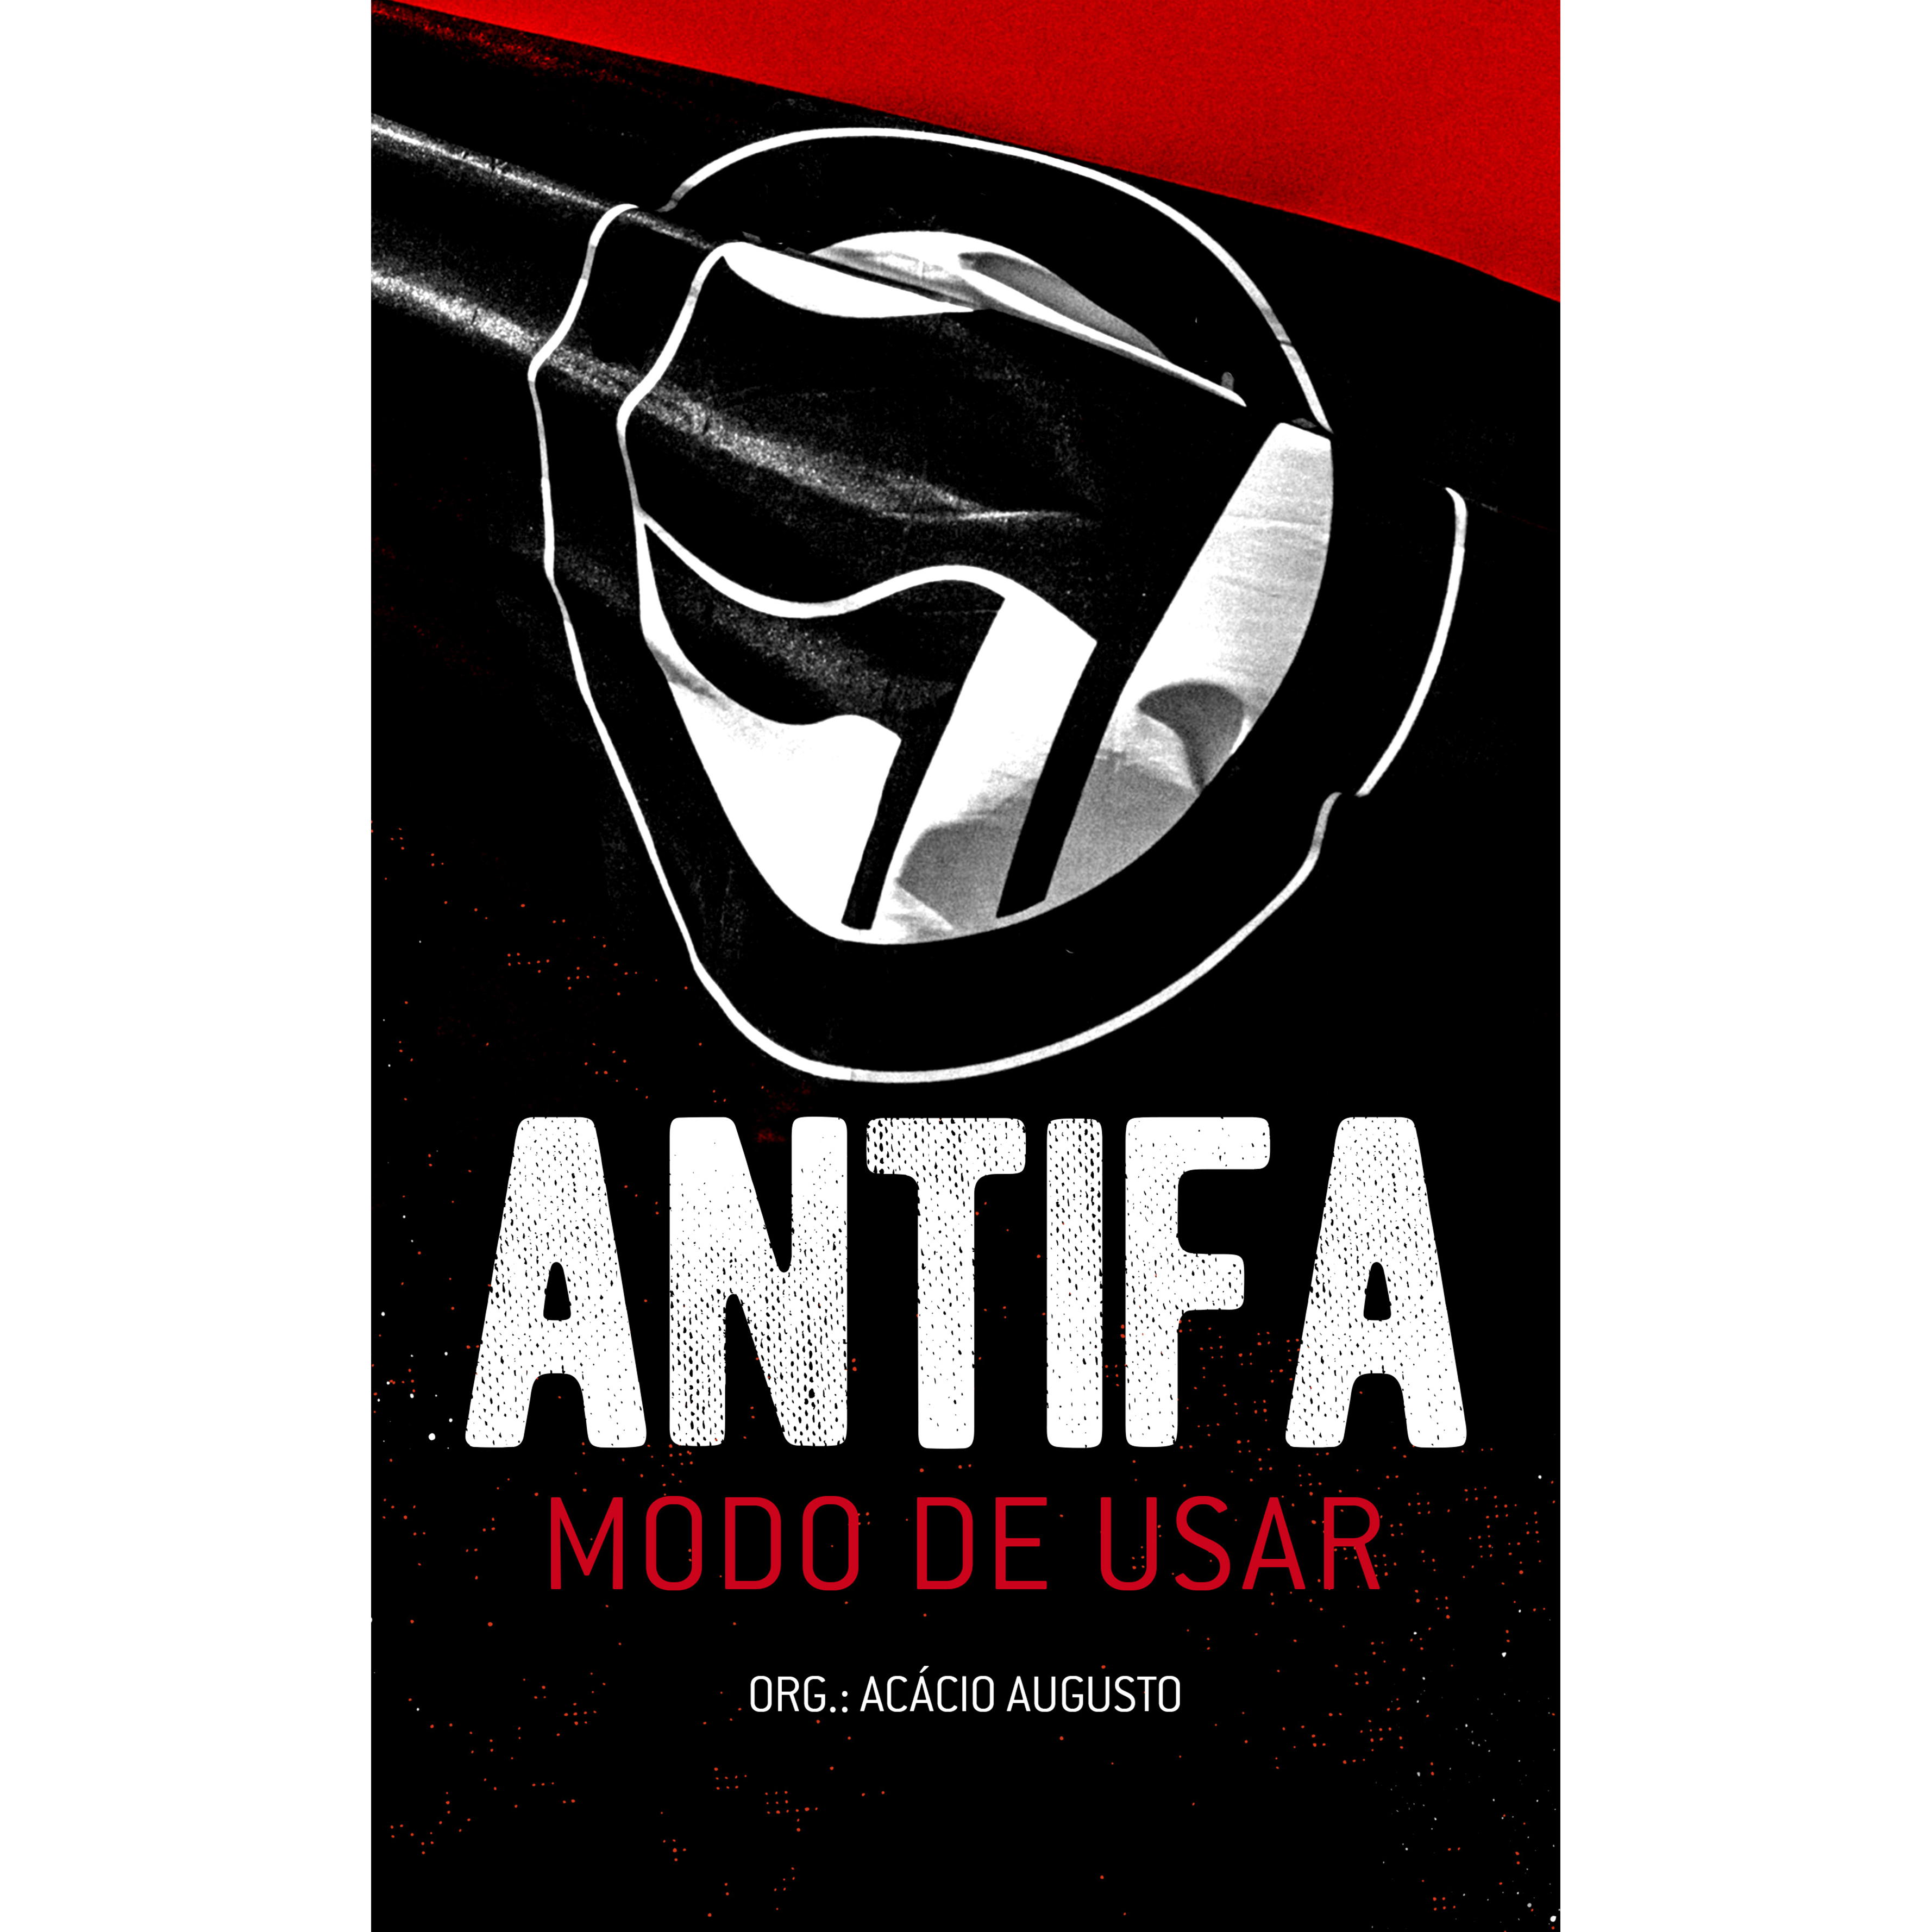
\includegraphics[width=74mm]{./grid/antifa.png}
\end{center}

\hspace*{-7cm}\hrulefill\hspace*{-7cm}

\medskip

\noindent{}A ascensão ao poder de uma direita radicalizada, nova sobretudo nos métodos de ação e no uso eficiente das tecnologias modernas, impõe uma reflexão de ordem tática: o que é, hoje, o antifascismo? Como a convulsão social pode organizar"-se contra o controle imposto por polícias ultraviolentas?
Se por um lado governantes como Jair Bolsonaro ou Donald Trump dispõem de amplo arsenal fático e bélico, a explosão recente de protestos pelo mundo aponta para uma janela de ação, em que a revolta popular também se radicaliza e, literalmente, coloca nações inteiras em chamas.

E é na esteira desse momento fundamental que é estruturado {\slsc{Antifa: modo de usar}}. A publicação reúne ensaios, textos e entrevistas do historiador americano Mark Bray, especialista no movimento antifascista e uma das principais vozes do momento de luta. Além de textos de Acácio Augusto --- organizador do volume, cientista social e pesquisador em estudos libertários do grupo Nu-Sol --- compondo um material urgente e essencial para nosso tempo.

\vfill

\hspace*{-.4cm}\begin{minipage}[c]{.5\linewidth}
\small{
{\Formular{\textbf{
\hspace*{-.1cm}\hlc[lightyellow]{Editora: Circuito \& Hedra}\\
Título: Antifa: modo de usar\\
Autor: Acácio Augusto (org.)\\ 
ISBN: 978-85-7715-652-8\\
Páginas: ???\\
Formato: 12,7x19,1cm\\
Preço: R\$ ????\\
Disponibilidade: 17/07/2020
}}}}
\end{minipage}

\pagebreak %INTRODUÇÃO À SOMA

\begin{center}
\hspace*{.5cm}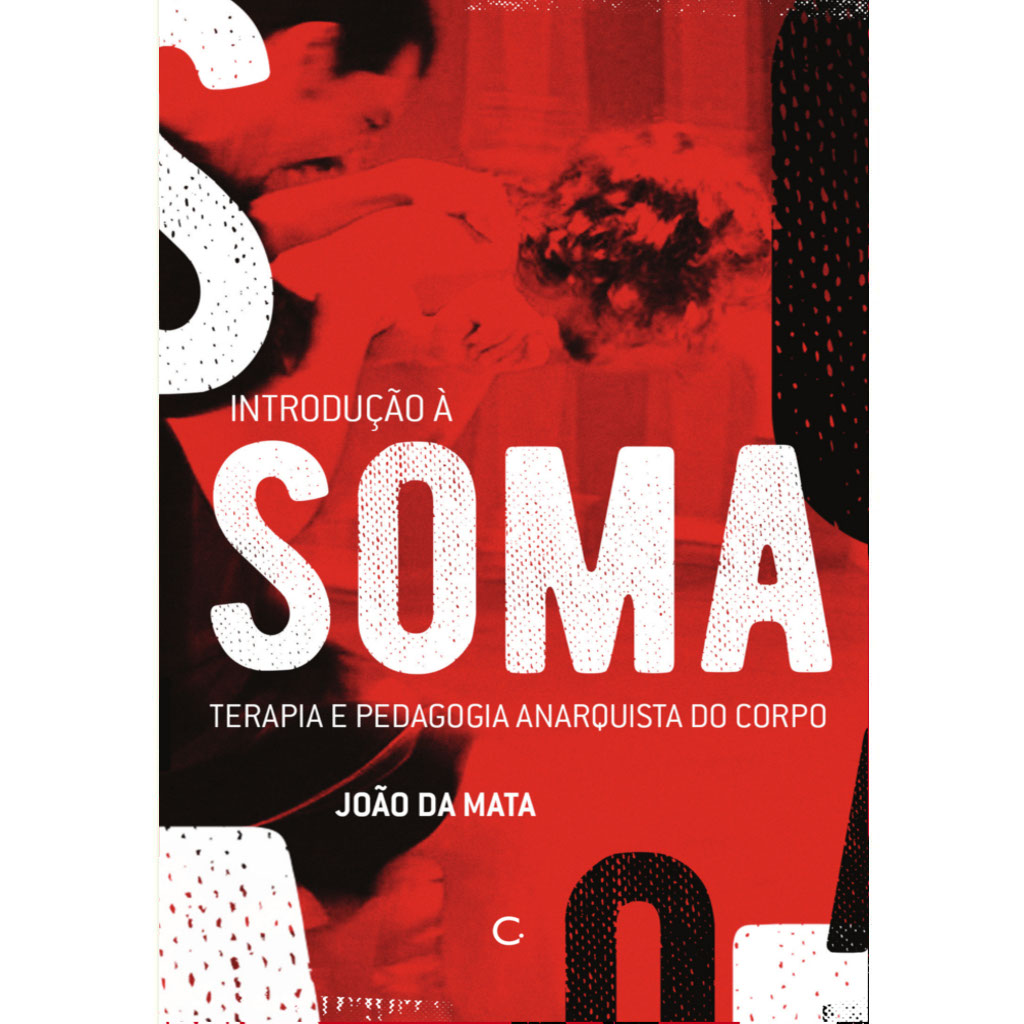
\includegraphics[width=74mm]{./grid/soma.png}
\end{center}

\hspace*{-7cm}\hrulefill\hspace*{-7cm}

\medskip

\noindent{}{\slsc{Introdução à Soma: terapia e pedagogia anarquista do corpo}} trata de um processo terapêutico corporal realizado em grupo, que busca no pensamento anarquista uma crítica às mais variadas formas de poder impregnadas no comportamento individual e nas relações sociais. O grupo de terapia funciona como um micro"-laboratório social, no qual se desenvolve uma análise libertária do comportamento de cada um a partir da relação junto ao outro.

Daí sua originalidade: terapia como criação e afirmação de si, em que a construção das práticas de liberdade é o antídoto para combater os conflitos gerados pelas relações sociais hierarquizadas. A somaterapia ou apenas Soma é um processo terapêutico"-pedagógico, realizado em grupo e com ênfase na articulação entre o trabalho corporal e o uso da linguagem verbal. Foi criada no Brasil pelo escritor e terapeuta Roberto Freire, a partir da obra de Wilhelm Reich e sua pesquisa sobre corpo e emoção.

\vfill

\hspace*{-.4cm}\begin{minipage}[c]{.5\linewidth}
\small{
{\Formular{\textbf{
\hspace*{-.1cm}\hlc[lightyellow]{Editora: Circuito \& Hedra}\\
Título: Introdução à Soma — terapia\\ e pedagogia anarquista do corpo\\
Autor: João da Mata\\ 
ISBN: 978-85-9582-055-5\\
Páginas: 106\\
Formato: 12,7x19,1cm\\
Preço: R\$ 42,90\\
Disponibilidade: 17/07/2020
}}}}
\end{minipage}

\pagebreak %FILOSOFIA BLACK BLOC

\begin{center}
\hspace*{-3.6cm}\raisebox{5cm}{\rotatebox[origin=t]{90}{\huge\Formular{\textbf{Lançamento}}}}
\hspace*{3.1cm}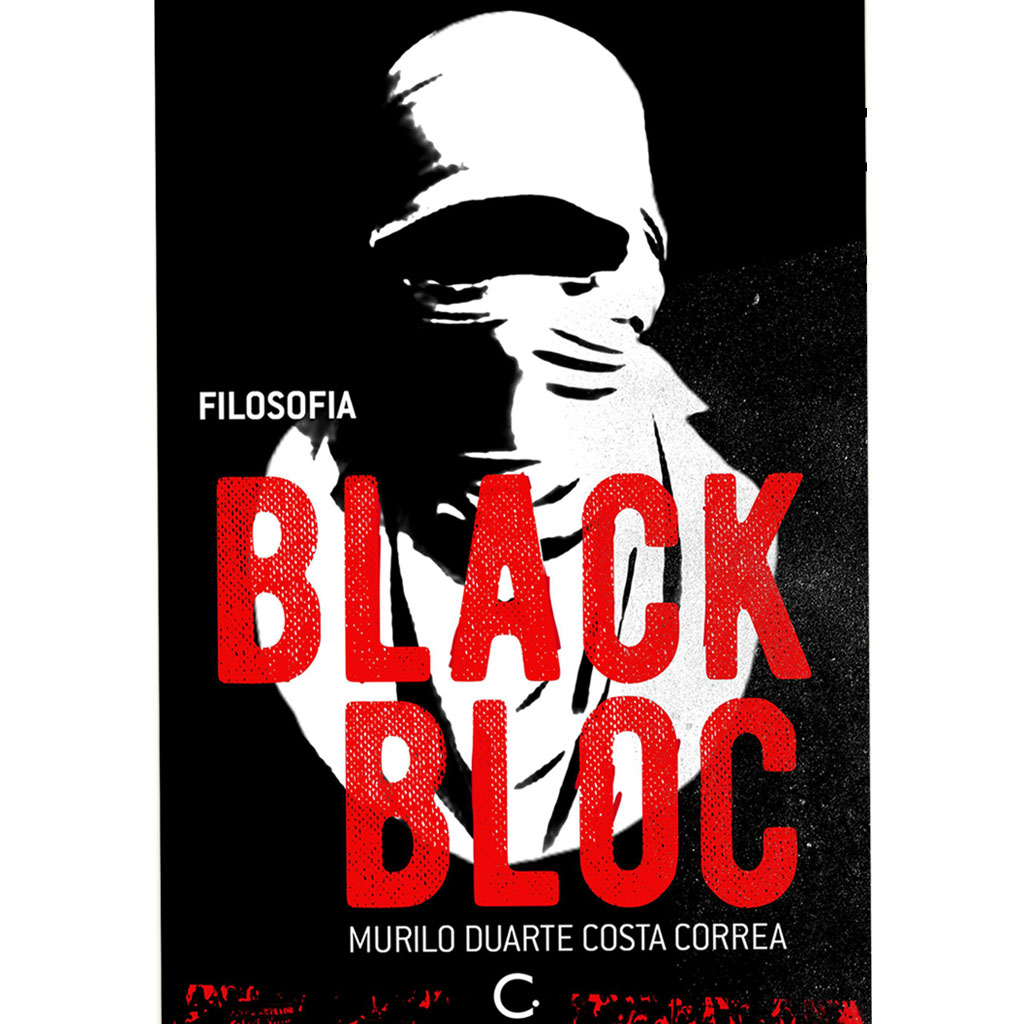
\includegraphics[width=74mm]{./grid/black.png}
\end{center}

\hspace*{-7cm}\hrulefill\hspace*{-7cm}

\medskip

\noindent{}Em junho de 2013, data da maior erupção social das últimas décadas, o movimento {\slsc{Black Bloc}} ganhou os holofotes como nova prática de luta e manifestação. Analistas à direita e à esquerda foram forçados a tentar compreender o movimento, normalmente municiando um repertório conceitual incompatível com os significados do {\slsc{Black Bloc}}, sem entendê"-lo em seus próprios termos.

Procurando suprir essa carência surge o {\slsc{Filosofia Black Bloc}}, que concebe e mobiliza um arcabouço teórico que permita abordar o movimento {\slsc{Black Bloc}} como fenômeno: produzir, no pensamento, uma filosofia {\slsc{Black Bloc}}. Não cessamos de ler Junho sob o ponto de vista de Brasília, dos palácios de governo, dos partidos recusados pelas multidões, da surpresa e da inércia dos poderes constituídos, da decadência da representação formal, das classes cerradas para o social. Pensar Junho nesses termos torna"-se então “capturar e destruir” sua potência específica. Não é por acaso que boa parte das interpretações de intelectuais se parece tanto com os discursos da grande imprensa que vimos circular.


\vfill

\hspace*{-.4cm}\begin{minipage}[c]{.5\linewidth}
\small{
{\Formular{\textbf{
\hspace*{-.1cm}\hlc[lightyellow]{Editora: Circuito \& Hedra}\\
Título: Filosofia Black Bloc\\
Autor: Murilo Duarte Costa Correa\\ 
ISBN: 978-85-9582-056-2\\
Páginas: 166\\
Formato: 12,7x19,1cm\\
Preço: R\$ 46,90\\
Disponibilidade: 17/07/2020
}}}}
\end{minipage}


\pagebreak %1967, MEIO SÉCULO DEPOIS


\begin{center}
\hspace*{.5cm}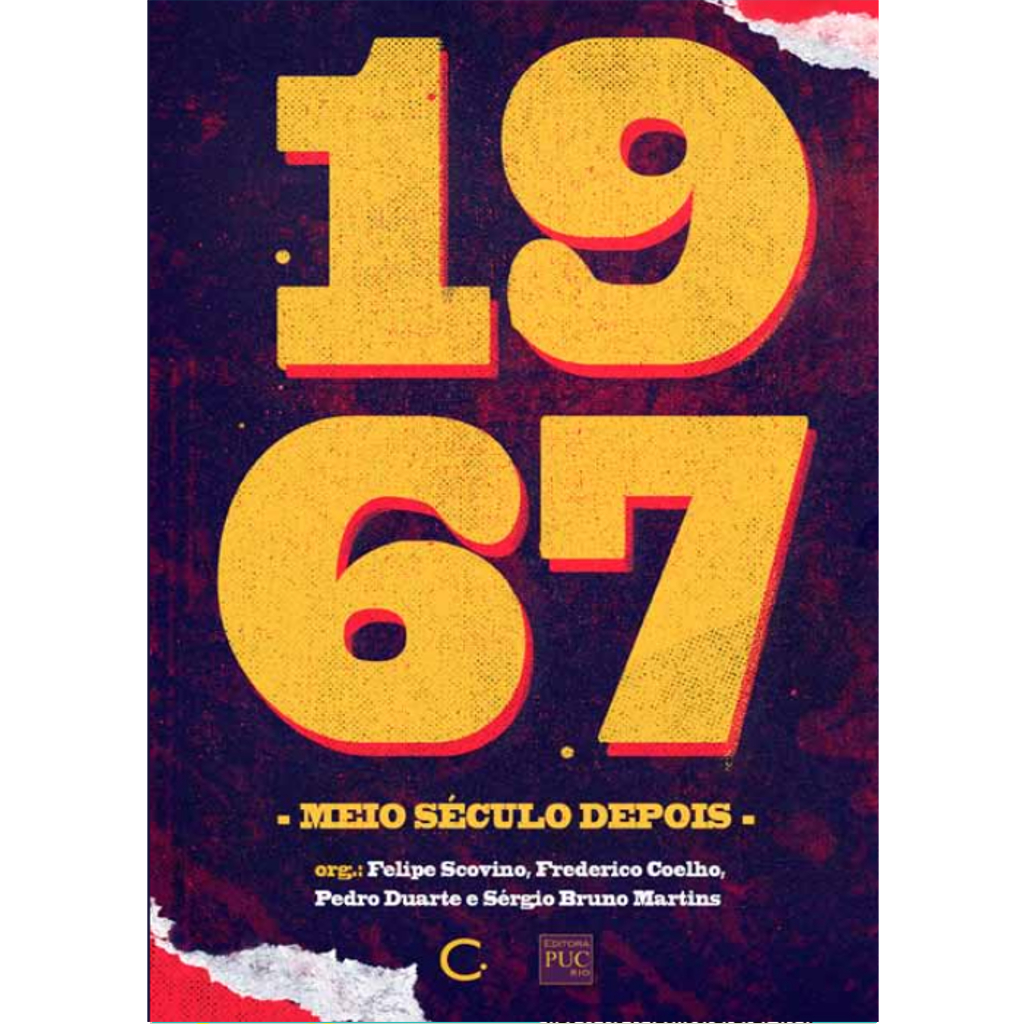
\includegraphics[width=74mm]{./grid/1967.png}
\end{center}

\hspace*{-7cm}\hrulefill\hspace*{-7cm}

\medskip

\noindent{}{\slsc{1967, meio século depois}} é um livro que sonda --- na confluência das artes plásticas, literatura, cinema, \scalebox{.8}{TV}, teatro e política --- o ano de 1967 e seus principais desdobramentos no pensamento e na cultura brasileira. Diversos ensaístas e intelectuais analisam no livro temas como o tropicalismo, os festivais de música, as revoluções perpetradas por Zé Celso no Teatro Oficina, o Cinema Novo de Glauber Rocha e as provocantes obras de Hélio Oiticica.

Às vésperas do período mais ditatorial e repressivo da história brasileira, as artes tentaram abrir  caminhos de liberdade e insurgência de um Brasil plurívoco e múltiplo, nos quais os autores procuram linhas de permanências e rupturas cinquenta anos depois. Como escreve Frederico Coelho, um dos organizadores do volume, fazer esse balanço serve de “alerta dentre as novas gerações cuja leitura pode cada vez mais se aproximar daquele momento dramático pela lente absurda de nosso presente”, em um tempo que a missão do intelectual é entender que “diagnósticos precários se tornaram parte de nosso cotidiano na luta contra a linha evolutiva do conservadorismo brasileiro”.


\vfill
\enlargethispage{\baselineskip}

\hspace*{-.4cm}\begin{minipage}[c]{1\linewidth}
\small{
{\Formular{\textbf{
\hspace*{-.1cm}\hlc[lightyellow]{Editora: Circuito \& Editora PUC-Rio}\\
Título: 1967, meio século depois\\
Autor: Felipe Scovino, Fred Coelho,\\ Pedro Duarte e Sérgio Martins (orgs.)\\ 
ISBN: 978-85-9582-057-9\\
Páginas: 268\\
Formato: 16x23cm\\
Preço: R\$ ????\\
Disponibilidade: 28/08/2020
}}}}
\end{minipage}

\pagebreak

\pagestyle{circuitocat}

\begin{multicols}{2}
\begin{enumerate}
\raggedright\nohyphens{
\item A grande marcha, {\Formular{\textbf{Ewerton Martins Ribeiro }}}
\item A loucura branca, {\Formular{\textbf{Jaime Rocha}}}
\item A outra morte de Alberto Caeiro, {\Formular{\textbf{Afonso Henriques Neto}}}
\item A Dialética do gosto, {\Formular{\textbf{Marco Scheinder}}}
\item Adoecer, {\Formular{\textbf{Hélia Correia}}}
\item Almas selvagens, {\Formular{\textbf{André Gardel}}}
\item Até ano que vem em Jerusalém, {\Formular{\textbf{Maria da Conceição Caleiro}}}
\item Cadernos de artista, {\Formular{\textbf{Moisés Alves}}}
\item Cérebro-Ocidente/Cérebro"-Brasil, {\Formular{\textbf{Roberto Corrêa dos Santos}}}
\item Nove tiros em Chef Lidu, {\Formular{\textbf{Paula Bajer Fernandes}}}
\item Comunidades sem fim
\item Coletivos
\item DJs
\item Dezembro, {\Formular{\textbf{Ana Tereza Salek}}}
\item Os tigres cravaram as garras no horizonte, {\Formular{\textbf{Augusto Guimaraens Cavalcanti}}}
\item No contemporâneo: arte e escritura expandidas, {\Formular{\textbf{Roberto Corrêa dos Santos; Renato Rezende}}}
\item Truques de autor, {\Formular{\textbf{Heleno Bernardi}}}
\item Clínica de artista I, {\Formular{\textbf{Roberto Corrêa dos Santos}}}
\item Clínica de artista II, {\Formular{\textbf{Roberto Corrêa dos Santos}}}
\item Vertigens, {\Formular{\textbf{Fernanda de Mello Gentil}}}
\item Nós somos uma correspondência, {\Formular{\textbf{Fernanda de Mello Gentil}}}
\item Amarração, {\Formular{\textbf{Renato Rezende}}}
\item Conversas com curadores e críticos de arte
\item Experiência e arte contemporânea
\item Romance, {\Formular{\textbf{Caio Meira}}}
\item Auréola, {\Formular{\textbf{Renato Rezende}}}
\item Cosmocrunch, {\Formular{\textbf{Maria Dolores Wanderley}}}
\item Preces para a amiga submersa, {\Formular{\textbf{Lucia Castello Branco}}}
\item Pequena coleção de grandes horrores, {\Formular{\textbf{Luiz Brás}}}
\item Nós, o outro, o distante na arte brasileira contemporânea, {\Formular{\textbf{Marisa Flórido Cesar}}}
\item Lira dos sentidos, {\Formular{\textbf{Carlos Henrique Costa}}}
\item Rasga-mortalha: poemas dos outros, {\Formular{\textbf{W. B. Lemos}}}
\item Os nomes, {\Formular{\textbf{Rogério Luz}}}
\item N’Ágorainda, {\Formular{\textbf{Naila Rachid}}}
\item O ser-se, {\Formular{\textbf{Júnia Azevedo}}}
\item A reflexão atuante, {\Formular{\textbf{Sergio Cohn}}}
\item Intervenções críticas, {\Formular{\textbf{Josefina Ludmer}}}
\item O homem mais portátil do mundo, {\Formular{\textbf{Arturo Carrera}}}
\item O capitão Nemo e eu, {\Formular{\textbf{Alfredo Prior}}}
\item Notas, disparos, sublinhados, {\Formular{\textbf{María Moreno}}}
\item Naxos, {\Formular{\textbf{Elsa Cross}}}
\item Diário em progresso, {\Formular{\textbf{Alex Frechette}}}
\item Em caso de emergência pare o tempo, {\Formular{\textbf{Gab Marcondes}}}
\item 1,68 x 1,81, {\Formular{\textbf{Maria André Leite}}}
\item Do tudo e do todo, {\Formular{\textbf{Cláudio Oliveira}}}
\item S.O.S. Poesia, {\Formular{\textbf{Renato Rezende; Dirk Vollenbroich}}}
\item O olho do lince, {\Formular{\textbf{Guilherme Zarvos}}}
\item Diário para descolorir, {\Formular{\textbf{Alex Frechette}}}
\item A pequena voz do mundo, {\Formular{\textbf{Diana Bellessi}}}
\item Amazônia \& Co., {\Formular{\textbf{Rafael Cippolini}}}
\item Fala, poesia, {\Formular{\textbf{Tamara Kamenszain}}}
\item Suturas. Um breviário, {\Formular{\textbf{Daniel Link}}}
\item Repetir, {\Formular{\textbf{Katia Maciel}}}
\item Coreografia (Orelhas contemporâneas), {\Formular{\textbf{André Parente}}}
\item Amor: verso: reverso (Orelhas contemporâneas), {\Formular{\textbf{Luiz Sérgio de }}}Oliveira
\item Saudades de um punhal (Orelhas contemporâneas), {\Formular{\textbf{Leila Danziger}}}
\item Gravidade (Orelhas contemporâneas), {\Formular{\textbf{Katia Maciel}}}
\item Artexperiência contemporânea (Orelhas contemporâneas), {\Formular{\textbf{Renato }}}Rezende
\item Práticas contemporâneas do mover-se, {\Formular{\textbf{Michelle Sommer}}}
\item Levantem lentamente o lençol, {\Formular{\textbf{Bia Albernaz}}}
\item Escritos sobre fotografia contemporânea brasileira
\item Doctypes, {\Formular{\textbf{Alex Hamburger}}}
\item Quarenta e quatro, {\Formular{\textbf{Mauricio Cardozo}}}
\item Ninfas e Mariposas, {\Formular{\textbf{Leonardo Toledo}}}
\item Lab Criativo / Creative Lab
\item Quase-poesia, {\Formular{\textbf{Jerson Lima Silva}}}
\item Música Chama, {\Formular{\textbf{Pedro Sá Moraes; Eduardo Guerreiro B. Losso}}}
\item Viventes de Saturno, {\Formular{\textbf{Carlos Frederico Manes}}}
\item Esperando a hora da Stella, {\Formular{\textbf{Maria Dolores Wanderley}}}
\item Falar o que seja é inútil – ou sobre desconsiderações, {\Formular{\textbf{Carlos Alberto Gianotti}}}
\item Lótus molotov, {\Formular{\textbf{Leonardo Toledo}}}
\item Outras margens, {\Formular{\textbf{Sergio Cohn}}}
\item Formas híbridas, {\Formular{\textbf{Rafael Gutiérrez}}}
\item Fornicar e matar e outros ensaios, {\Formular{\textbf{Laura Klein}}}
\item Cores cobras pincéis cães, {\Formular{\textbf{Eduardo Stupía}}}
\item Lasca de breu, {\Formular{\textbf{Guilherme Delgado}}}
\item O tropo tropicalista, {\Formular{\textbf{João Camillo Penna}}}
\item Leituras furadas, {\Formular{\textbf{Luis Felipe Fabre}}}
\item Escrever sobre escrever poesia, {\Formular{\textbf{Eduardo Milán}}}
\item A liberação da mosca, {\Formular{\textbf{Luigi Amara}}}
\item Mudança, {\Formular{\textbf{Verónica Gerber Bicecci}}}
\item Onde late um cachorro doido, {\Formular{\textbf{Moisés Alves}}}
\item Daniel Acosta
\item Éter, {\Formular{\textbf{António Cabrita}}}
\item Noturno Europeu, {\Formular{\textbf{Rui Nunes}}}
\item Café irlandês, {\Formular{\textbf{Barbosa Lagos}}}
\item Voo, {\Formular{\textbf{Ana Paula Simonaci}}}
\item Fim do Infante, {\Formular{\textbf{Marina Marcondes Machado}}}
\item 2013, memórias e resistências, {\Formular{\textbf{Camila Jourdan}}}
\item Escrito e dirigido por Moisés Alves, {\Formular{\textbf{Moisés Alves}}}
\item Coisas que fiz e ninguém notou mas que mudaram tudo, {\Formular{\textbf{Moisés Alves}}}
\item A cena lenta, {\Formular{\textbf{Cláudio Oliveira}}}
\item Copa pra quem? Olimpíadas pra quem?, {\Formular{\textbf{Alex Frechette}}}
\item O fantasma de um nome (poesia, imaginário, vida), {\Formular{\textbf{Jorge Monteleone}}}
\item Peso Morto, {\Formular{\textbf{João Felipe Gremski}}}
\item Romance de asilo, {\Formular{\textbf{André Monteiro}}}
\item Quem apaga a luz sou eu, {\Formular{\textbf{Magda Romano}}}
\item As artes do cover, {\Formular{\textbf{Henrique Saidel}}}
\item Frestas, {\Formular{\textbf{André Gardel}}}
\item O antes é o depois, {\Formular{\textbf{Guidi Vieira}}}
\item Humano, {\Formular{\textbf{Pedro Poeta}}}
}
\end{enumerate}
\end{multicols}

\pagebreak
